\chapter{Separar mezclas}\label{ch:g3:separating-mixtures}

Después de una tormenta, los charcos del camino son marrones: agua de
lluvia \omterm{def:g2:mixing-and-dissolving:mix}{mezclada} con tierra, arena y trocitos de hojas. Sin embargo, el
agua que sale del grifo de la cocina es transparente, y también fue
lluvia antes de llegar a un río. ¿Cómo se puede volver a limpiar el agua
turbia? Lo que se ha \omterm{def:g2:mixing-and-dissolving:mix}{mezclado} se puede separar. Este capítulo enseña
cómo hacerlo, método a método.

\begin{recall}
\omterm{def:g2:mixing-and-dissolving:mix}{Mezclar} es juntar cosas distintas. Un sólido como el azúcar o la sal se
\omterm{def:g2:mixing-and-dissolving:dissolve}{disuelve} en agua: desaparece de la vista, y el líquido transparente es
una disolución. Un sólido disuelto sigue ahí: cuando el agua se seca,
el sólido se queda. La arena y la tierra no se \omterm{def:g2:mixing-and-dissolving:dissolve}{disuelven}
(\cref{ch:g2:mixing-and-dissolving}).
\end{recall}

\section{Separar a mano y tamizar}

Cuando los trozos de una mezcla son lo bastante grandes para verlos y
cogerlos, la forma más sencilla de separarlos es a mano: las pasas se
pueden sacar del muesli una a una. Cuando hay demasiados trozos, un
tamiz hace el trabajo por nosotros.

\begin{definition}[Tamizado]\label{def:g3:separating-mixtures:sieve}
El \emph{tamizado}\index{tamizado} consiste en separar los trozos de
una mezcla según su tamaño, con un tamiz: una malla o una placa llena
de agujeros. Los trozos pequeños caen por los agujeros; los grandes se
quedan en el tamiz.
\end{definition}

\begin{example}[Grava y arena]\label{ex:g3:separating-mixtures:gravel}
Un albañil sacude una mezcla de grava y arena sobre un tamiz. La arena
fina cae y forma un montón debajo; la grava se queda en la malla.
\end{example}

\begin{omfigure}
\begin{tikzpicture}[font=\small]
  % the sieve: a mesh bowl
  \fill[pattern=crosshatch, pattern color=black!45] (-1.6,2.6) arc[start angle=180,
    end angle=360, x radius=1.6, y radius=0.7] -- cycle;
  \draw[black!70, line width=0.8pt] (-1.6,2.6) arc[start angle=180, end angle=360,
    x radius=1.6, y radius=0.7];
  \draw[black!70, line width=0.8pt] (-1.75,2.6) -- (1.75,2.6);
  \draw[black!70, line width=1.4pt] (1.75,2.6) -- (3.0,2.85);
  % gravel kept in the sieve
  \foreach \x/\y/\r in {-0.9/2.25/0.17,-0.45/2.12/0.2,0.05/2.08/0.18,0.5/2.13/0.21,
                        0.95/2.28/0.16,-0.2/2.42/0.15,0.3/2.43/0.17}
    \fill[black!45, draw=black!65] (\x,\y) circle (\r);
  % sand falling
  \foreach \x/\y in {-0.4/1.6,0.1/1.4,0.4/1.7,-0.15/1.15,0.25/1.0,-0.5/0.95,0.0/0.75}
    \fill[orange!60!brown] (\x,\y) circle (0.05);
  % the heap of sand in a bowl
  \fill[orange!45!brown!70] (-1.0,0.12) .. controls (-0.5,0.55) and (0.5,0.55)
    .. (1.0,0.12) -- cycle;
  \draw[black!70, line width=0.8pt] (-1.5,0.5) .. controls (-1.3,0) and (1.3,0)
    .. (1.5,0.5);
  \node[anchor=west] at (2.0,2.2) {la grava se queda en el tamiz};
  \node[anchor=west] at (2.0,1.25) {la arena cae por los agujeros};
  \node[anchor=west] at (2.0,0.3) {un montón de arena};
\end{tikzpicture}

{\small \omterm{def:g3:separating-mixtures:sieve}{Tamizado} de una mezcla de grava y arena: los trozos se separan
según su tamaño.}
\end{omfigure}

\begin{omfigure}
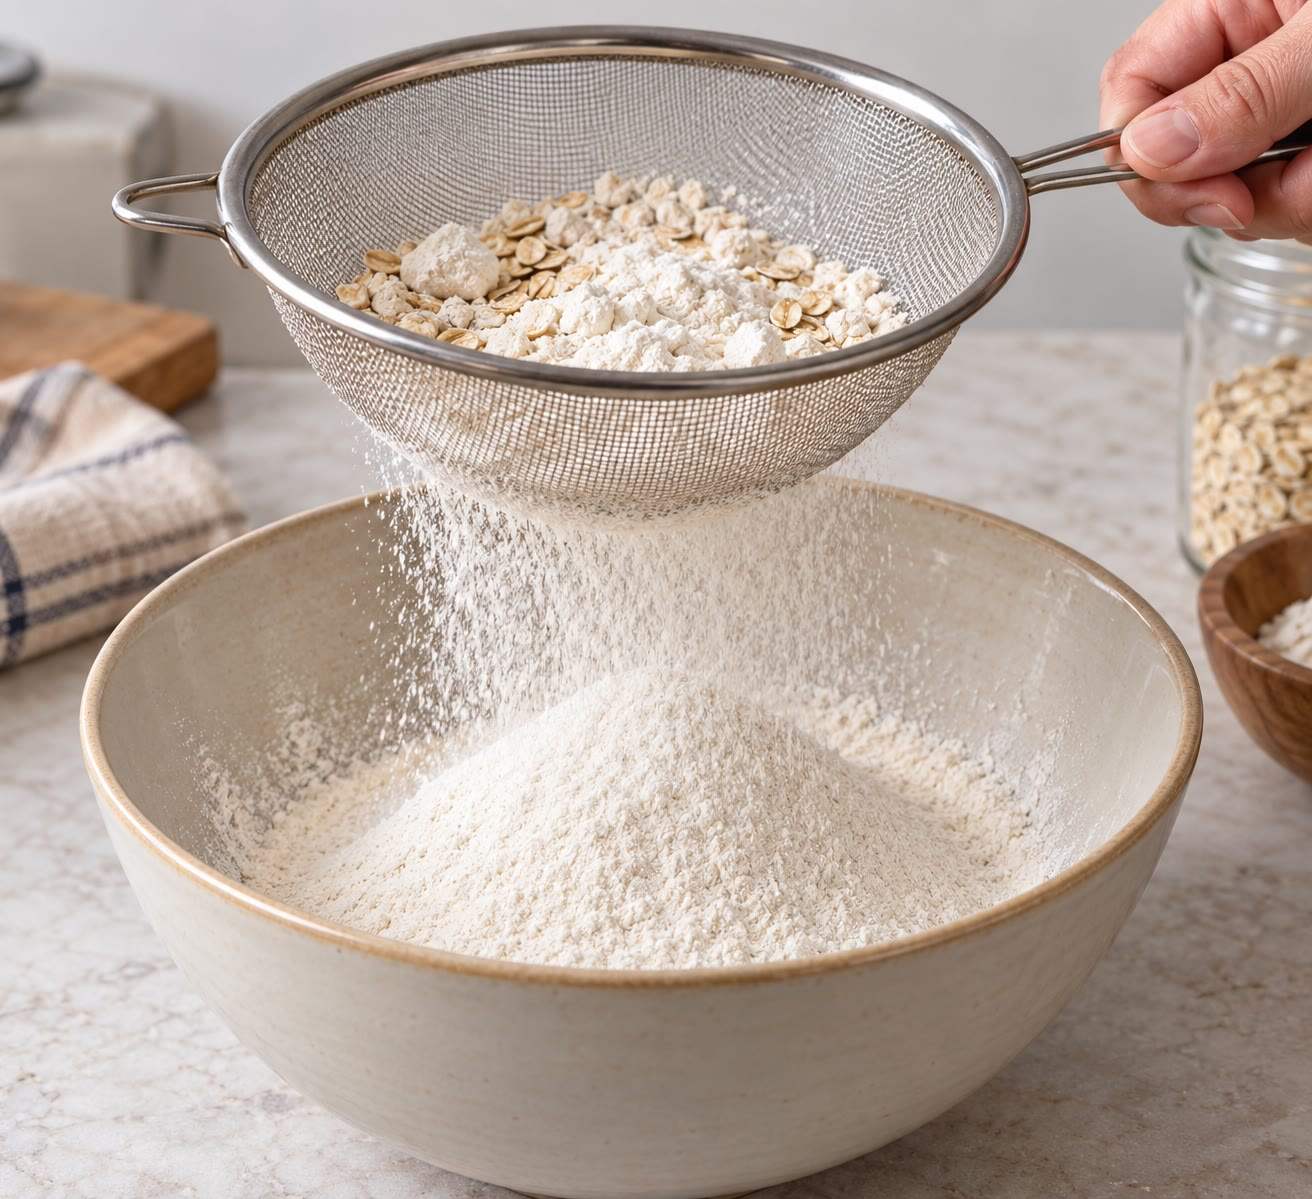
\includegraphics[width=0.55\linewidth]{images/book1/ai/g3-kitchen-sieve.jpg}

{\small Un colador de cocina: la harina fina pasa y los grumos se quedan.}
\end{omfigure}

\section{Dejar sedimentar y decantar}

\begin{definition}[Sedimentación y decantación]\label{def:g3:separating-mixtures:decant}
Una mezcla de agua y de un sólido que no se \omterm{def:g2:mixing-and-dissolving:dissolve}{disuelve} se puede dejar en
reposo: el sólido baja despacio hasta el fondo. Esto se llama
\emph{sedimentación}\index{sedimentacion@sedimentación}. Una vez sedimentado el
sólido, el agua transparente de encima se puede verter con cuidado en
otro recipiente, dejando atrás el sólido: esto es la
\emph{decantación}\index{decantacion@decantación}.
\end{definition}

\begin{omfigure}
\begin{tikzpicture}[font=\small]
  % 1: stirred, cloudy
  \pic at (0,0) {beaker={0.7}{brown!28}};
  \foreach \x/\y in {-0.5/0.3,-0.2/0.6,0.3/0.4,0.5/0.9,-0.4/1.0,0.1/1.2,0.4/0.15,
                     -0.1/0.25,0.2/0.8,-0.55/0.7}
    \fill[brown!60] (\x,\y) circle (0.03);
  \node[anchor=north, align=center] at (0,-0.15) {removida:\\ turbia};
  \draw[->, thick, omProp] (1.1,1.0) -- (2.4,1.0);
  % 2: settled
  \pic at (3.5,0) {beaker={0.7}{omWater!80}};
  \fill[brown!60] (2.7,0) rectangle (4.3,0.25);
  \draw[omGlass, line width=0.7pt] (2.7,0.25) -- (2.7,0) -- (4.3,0) -- (4.3,0.25);
  \node[anchor=north, align=center] at (3.5,-0.15) {en reposo:\\ la tierra se ha sedimentado};
  \draw[->, thick, omProp] (4.6,1.0) -- (5.9,1.0);
  % 3: decanted
  \pic at (7.0,0) {beaker={0.1}{omWater!80}};
  \fill[brown!60] (6.2,0) rectangle (7.8,0.25);
  \draw[omGlass, line width=0.7pt] (6.2,0.25) -- (6.2,0) -- (7.8,0) -- (7.8,0.25);
  \pic at (9.2,0) {beaker={0.58}{omWater!80}};
  \node[anchor=north, align=center] at (8.1,-0.15) {trasvasada: agua transparente\\ a la derecha, la tierra se queda};
\end{tikzpicture}

{\small \omterm{def:g3:separating-mixtures:decant}{Sedimentación} y después \omterm{def:g3:separating-mixtures:decant}{decantación} de una mezcla de tierra y
agua.}
\end{omfigure}

\begin{remark}[La sedimentación lleva tiempo]\label{rem:g3:separating-mixtures:time}
Los granos grandes y pesados se sedimentan en unos minutos; la arcilla
muy fina puede tardar un día o más, y mientras tanto el agua sigue un
poco turbia. La \omterm{def:g3:separating-mixtures:decant}{decantación} nunca quita todos los granos: con el agua
se va también un poco de turbidez.
\end{remark}

\section{Filtrar}

\begin{definition}[Filtración y filtrado]\label{def:g3:separating-mixtures:filter}
La \emph{filtración}\index{filtracion@filtración} consiste en verter una mezcla a
través de un filtro: una hoja de papel, una tela o una capa de arena con
agujeros demasiado pequeños para dejar pasar los trozos sólidos. El
sólido se queda en el filtro; el líquido transparente que lo atraviesa
se llama
\emph{filtrado}\index{filtrado}.
\end{definition}

\begin{omfigure}
\begin{tikzpicture}[font=\small, scale=1.4]
  \pic[transform shape] at (0,0) {beaker={0.35}{omWater!80}};
  \pic[transform shape] at (0,1.4) {funnel={brown!55}};
  % muddy water waiting in the paper cone, above the soil
  \fill[brown!25] (-0.411,2.45) -- (0.411,2.45) -- (0.722,2.8) -- (-0.722,2.8) -- cycle;
  % drops of filtrate
  \foreach \y in {1.15,0.95} \fill[omDef!50] (0,\y) circle (0.04);
  \draw[<-, omProp, thick] (0.75,2.6) -- (2.0,2.9) node[right, text=black]
    {papel de filtro en un embudo};
  \draw[<-, omProp, thick] (0.25,2.15) -- (2.0,2.2) node[right, text=black]
    {la tierra se queda en el papel};
  \draw[<-, omProp, thick] (0.85,0.4) -- (2.0,0.6) node[right, text=black]
    {el filtrado: agua transparente};
\end{tikzpicture}

{\small \omterm{def:g3:separating-mixtures:filter}{Filtración} de agua turbia con un filtro de papel.}
\end{omfigure}

\begin{inthelab}[Filtrar agua turbia]
El profesor dobla en forma de cono una hoja redonda de papel de filtro
y la coloca en un embudo de vidrio, encima de un vaso de precipitados.
Se vierte el agua turbia en el cono, poco a poco, sin pasar nunca del
borde del papel. El agua transparente gotea en el vaso; la tierra forma
una capa marrón sobre el papel. Si el \omterm{def:g3:separating-mixtures:filter}{filtrado} sale turbio, es que el
papel está roto o que el agua ha rebosado por su borde.
\end{inthelab}

\begin{proposition}[Un filtro no detiene lo que está disuelto]\label{prop:g3:separating-mixtures:dissolved}
Un filtro retiene los trozos sólidos que no están disueltos. No retiene
lo que está disuelto: el agua salada que se vierte por un filtro sale
igual de salada, y el té con azúcar, igual de dulce.
\end{proposition}

\begin{omfigure}
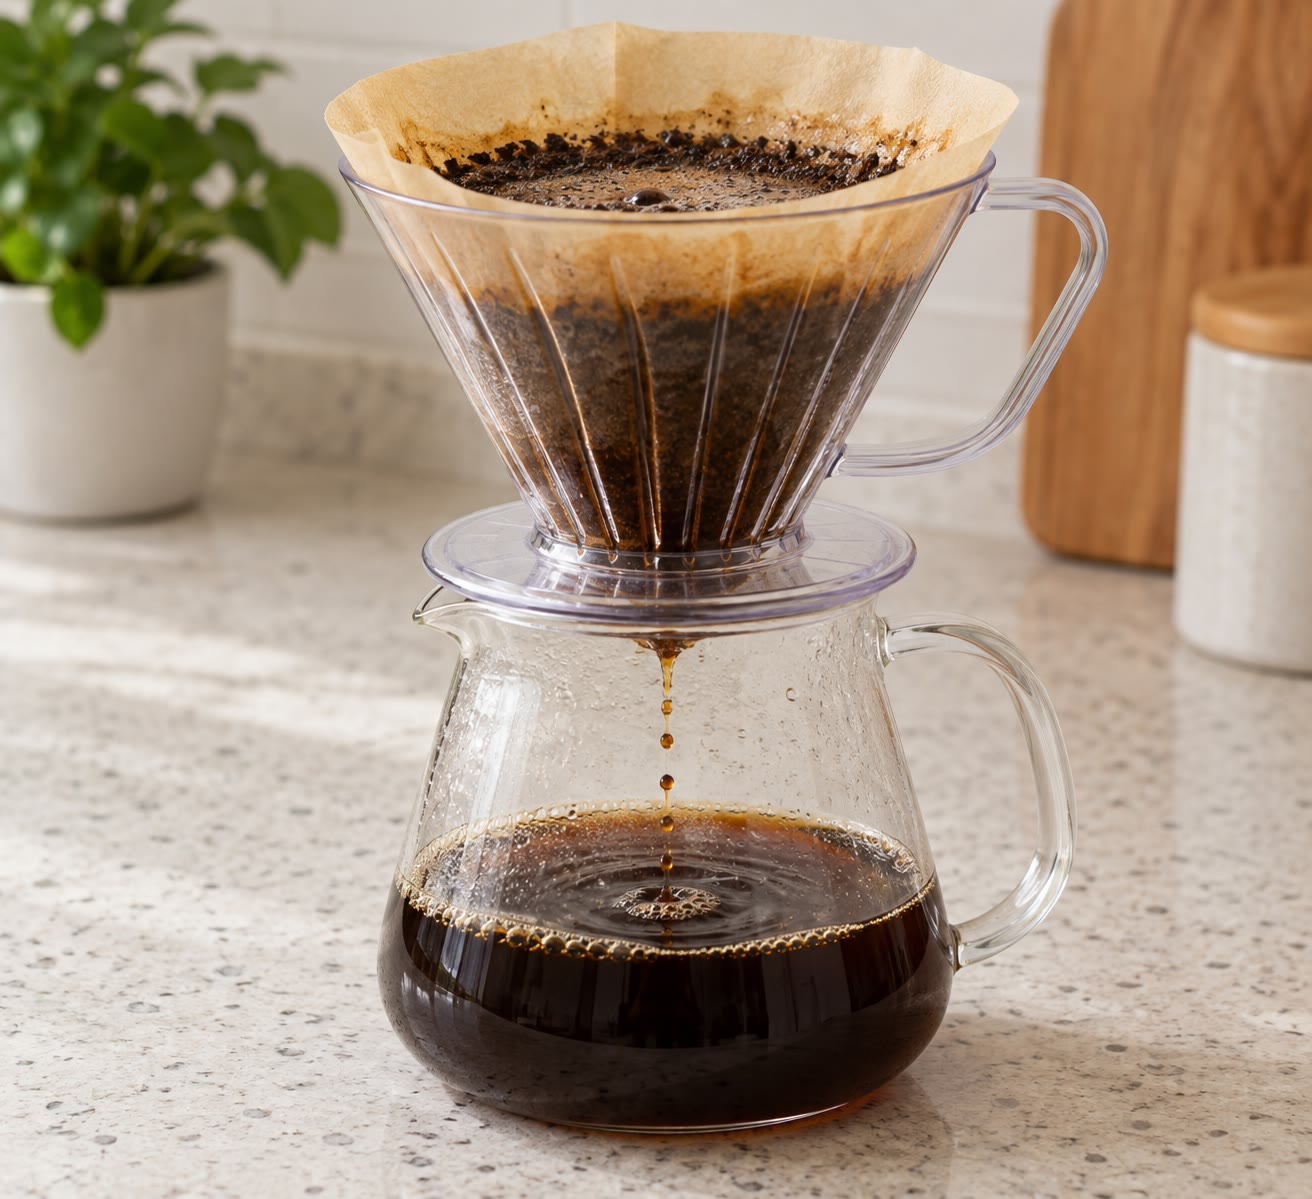
\includegraphics[width=0.5\linewidth]{images/book1/ai/g3-coffee-filter.jpg}

{\small Hacer café es filtrar: los posos se quedan en el papel y el café
es el \omterm{def:g3:separating-mixtures:filter}{filtrado}.}
\end{omfigure}

\section{Evaporar el agua}

\begin{definition}[Evaporación]\label{def:g3:separating-mixtures:evaporate}
Para recuperar un sólido disuelto en agua, se deja que el agua se seque,
al sol o con un calor suave: esto es la
\emph{evaporación}\index{evaporacion@evaporación}. El agua pasa al aire; el sólido
se queda en el recipiente.
\end{definition}

\begin{example}[Sal a partir de agua salada]\label{ex:g3:separating-mixtures:salt}
Se vierte un poco de agua salada en un recipiente poco hondo y se deja
en el alféizar de una ventana soleada. Días después ya no queda agua,
solo una costra blanca de sal: la sal que estaba disuelta.
\end{example}

\begin{omfigure}
\begin{tikzpicture}[font=\small, scale=1.4]
  \pic[transform shape] at (0,0) {hotplate};
  \pic[transform shape] at (0,0) {evapdish={omWater!80}};
  \node[anchor=north, align=center] at (0,-0.6) {agua salada,\\ calentada suavemente};
  \draw[->, thick, omProp] (1.5,0.3) -- (3.0,0.3) node[midway, above, text=black]
    {después};
  \pic[transform shape] at (4.5,0) {hotplate};
  \pic[transform shape] at (4.5,0) {evapdish={white!85!black}};
  \foreach \x in {-0.45,-0.25,-0.05,0.15,0.35}
    \fill[white, draw=black!45, line width=0.2pt] (4.5+\x,0.12) rectangle ++(0.09,0.06);
  \node[anchor=north, align=center] at (4.5,-0.6) {ya no queda agua:\\ cristales de sal};
  \foreach \x in {-0.3,0,0.3} \draw[->, black!45, decorate,
    decoration={snake, amplitude=0.6pt, segment length=4pt}] (\x,0.7) -- (\x,1.4);
  \node[anchor=south] at (0,1.4) {el agua pasa al aire};
\end{tikzpicture}

{\small La \omterm{def:g3:separating-mixtures:evaporate}{evaporación} en el laboratorio: el profesor calienta
suavemente el recipiente sobre una placa calefactora. La sal se queda en
el recipiente.}
\end{omfigure}

\section{¿Qué método para cada mezcla?}

\begin{method}[Elegir una separación]\label{met:g3:separating-mixtures:choose}
Para separar una mezcla, pregúntate:
\begin{enumerate}
  \item ¿Los trozos son grandes y de tamaños distintos? Sepáralos a mano,
        o tamízalos.
  \item ¿Hay un sólido que no se \omterm{def:g2:mixing-and-dissolving:dissolve}{disuelve} dentro de un líquido? Déjalo
        sedimentar y decanta, o filtra para obtener un agua más
        transparente.
  \item ¿Hay un sólido disuelto en el líquido? \omterm{def:g3:separating-mixtures:evaporate}{Evapora} el líquido: el
        sólido se queda.
\end{enumerate}
A menudo hacen falta varios pasos, uno detrás de otro.
\end{method}

\begin{example}[Arena, sal y agua]\label{ex:g3:separating-mixtures:three}
Un tarro contiene agua con arena y sal. La sal se ha disuelto; la arena,
no.
\begin{enumerate}
  \item Filtramos: la arena se queda en el papel.
  \item El \omterm{def:g3:separating-mixtures:filter}{filtrado} es transparente, pero es agua salada. La evaporamos:
        la sal se queda en el recipiente.
\end{enumerate}
Dos métodos, uno detrás de otro, nos devuelven la arena y la sal.
\end{example}

\begin{example}[Agua limpia a partir de un río]\label{ex:g3:separating-mixtures:plant}
Una planta potabilizadora convierte el agua del río en agua apta para
beber en varios pasos:
\begin{enumerate}
  \item el agua del río pasa por unas rejas, grandes rejillas que
        detienen ramas, hojas y plásticos: una especie de \omterm{def:g3:separating-mixtures:sieve}{tamizado};
  \item reposa en grandes depósitos donde el barro se sedimenta en el
        fondo;
  \item se filtra a través de gruesas capas de arena que retienen los
        granos más finos;
  \item se le añade una cantidad muy pequeña de un producto que mata los
        microbios, para que el agua siga siendo segura en las tuberías.
\end{enumerate}
\end{example}

\begin{omfigure}
\begin{tikzpicture}[font=\small, node distance=0.45cm,
    box/.style={draw=omDef, fill=omDef!6, rounded corners=2pt, align=center,
      minimum height=1.15cm, text width=2.0cm}]
  \node[box] (r) {agua\\ del río};
  \node[box, right=of r] (s) {rejas\\ (tamizado)};
  \node[box, right=of s] (t) {balsas de\\ decantación};
  \node[box, right=of t] (f) {filtros\\ de arena};
  \node[box, right=of f] (g) {microbios\\ eliminados};
  \foreach \a/\b in {r/s,s/t,t/f,f/g} \draw[->, thick, omProp] (\a) -- (\b);
  \node[below=0.15cm of s, font=\footnotesize, align=center] {ramas,\\ plásticos};
  \node[below=0.15cm of t, font=\footnotesize, align=center] {barro};
  \node[below=0.15cm of f, font=\footnotesize, align=center] {granos finos};
  \draw[->, thick, omProp] (g.south) -- ++(0,-0.8) node[below] {hacia los grifos};
\end{tikzpicture}

{\small Los pasos de una planta potabilizadora. Debajo de cada paso, lo
que elimina.}
\end{omfigure}

\begin{omfigure}
\begin{minipage}[t]{0.48\linewidth}\centering
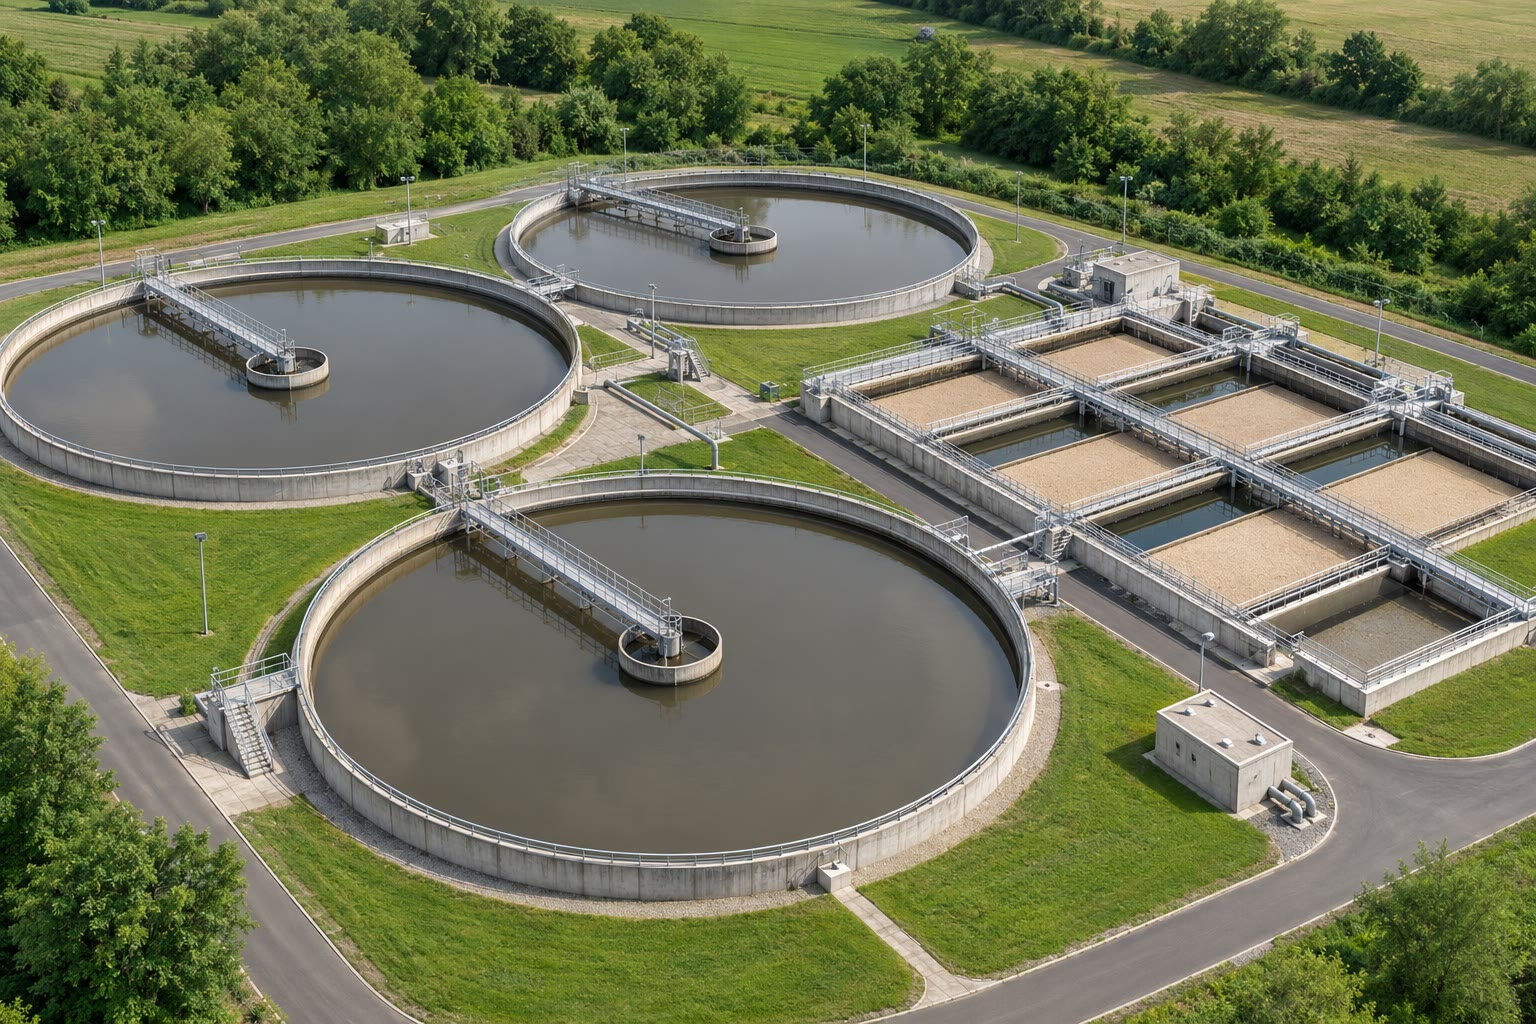
\includegraphics[width=\linewidth,height=4.6cm,keepaspectratio]{images/book1/ai/g3-settling-tanks.jpg}

{\small Depósitos de \omterm{def:g3:separating-mixtures:decant}{sedimentación} de una planta potabilizadora.}
\end{minipage}\hfill
\begin{minipage}[t]{0.48\linewidth}\centering
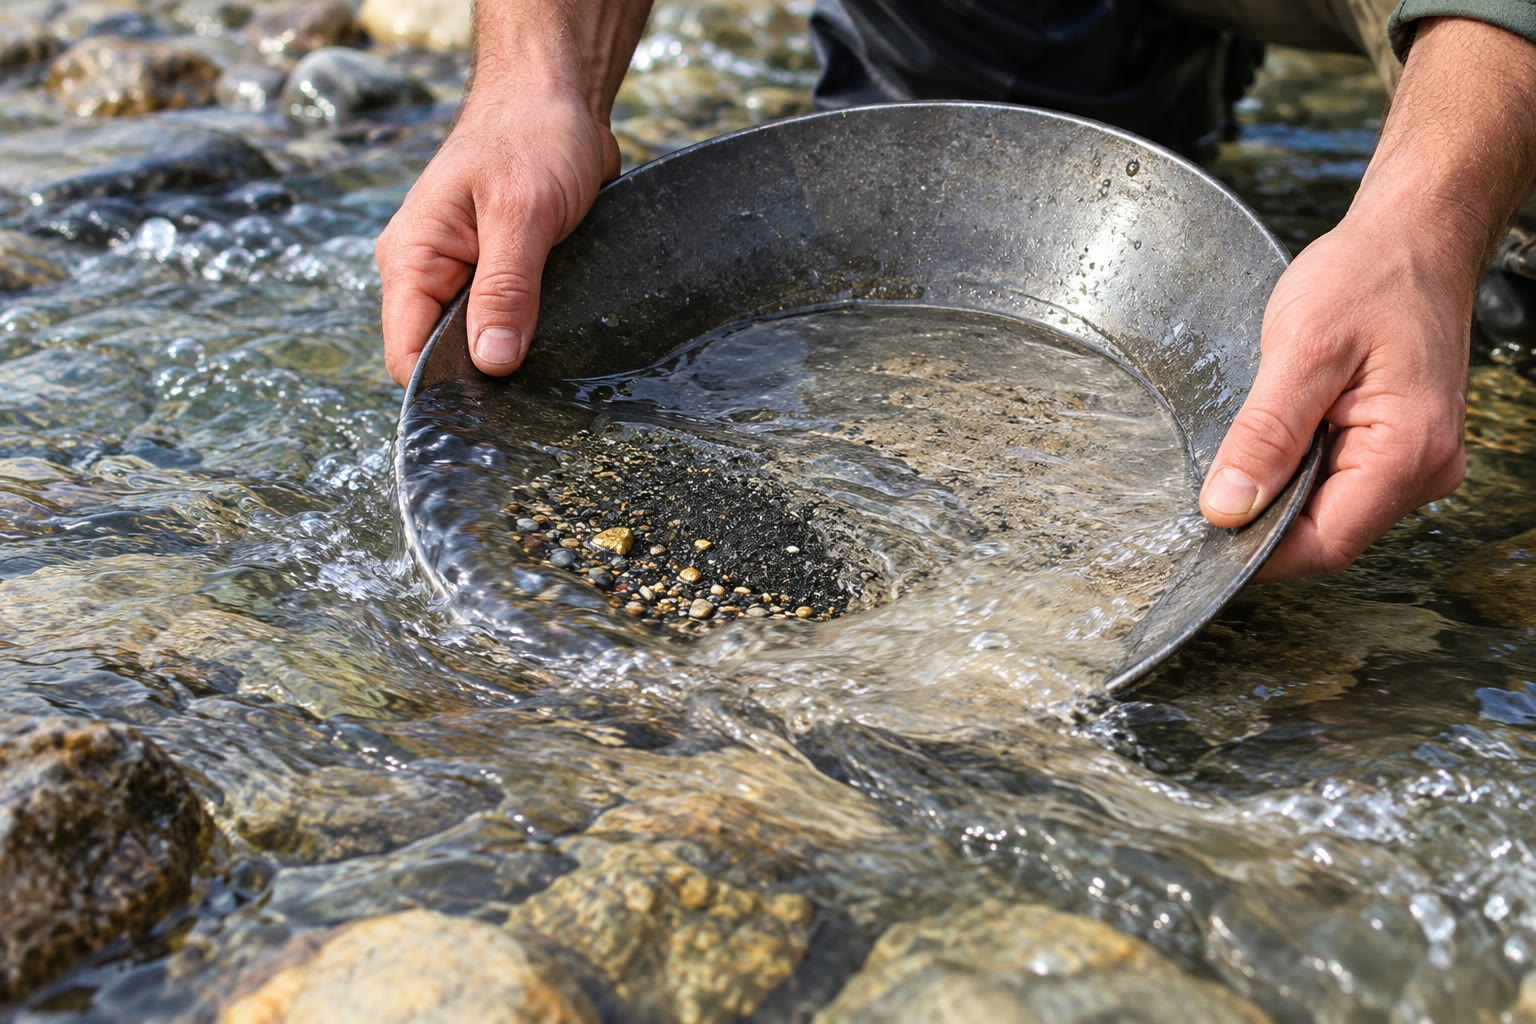
\includegraphics[width=\linewidth,height=4.6cm,keepaspectratio]{images/book1/ai/g3-gold-panning.jpg}

{\small Bateo de oro: el agua del río se lleva la arena ligera y los
granos pesados se quedan en la batea.}
\end{minipage}
\end{omfigure}

\begin{remark}[Transparente no siempre es limpio]\label{rem:g3:separating-mixtures:clean}
El agua filtrada puede parecer perfectamente transparente y contener
todavía sustancias disueltas, y microbios demasiado pequeños para
verlos. Por eso nadie bebe agua de un charco o de un arroyo, ni
siquiera después de filtrarla.
\end{remark}

\section{Ejercicios}

\begin{exercise}[$\star$]\label{exo:g3:separating-mixtures:1}
¿Qué método usarías para separar unos guisantes de unos granos de arroz?
\end{exercise}

\begin{exercise}[$\star$]\label{exo:g3:separating-mixtures:2}
Dejamos un vaso de agua turbia sobre una mesa durante una hora. ¿Qué le
pasa a la tierra? ¿Cómo se llama esto?
\end{exercise}

\begin{exercise}[$\star$]\label{exo:g3:separating-mixtures:3}
¿Qué es un \omterm{def:g3:separating-mixtures:filter}{filtrado}? Di cuál es el \omterm{def:g3:separating-mixtures:filter}{filtrado} cuando se hace café.
\end{exercise}

\begin{exercise}[$\star$]\label{exo:g3:separating-mixtures:4}
Vertemos agua salada a través de un papel de filtro. ¿El \omterm{def:g3:separating-mixtures:filter}{filtrado} es
salado? Explícalo.
\end{exercise}

\begin{exercise}[$\star$]\label{exo:g3:separating-mixtures:5}
¿Cómo se puede recuperar el azúcar de un vaso de agua con azúcar?
\end{exercise}

\begin{exercise}[$\star$]\label{exo:g3:separating-mixtures:6}
Mira la figura del tamiz. ¿Qué trozos se quedan en el tamiz? ¿Por qué
caen los demás?
\end{exercise}

\begin{exercise}[$\star$]\label{exo:g3:separating-mixtures:7}
Relaciona cada mezcla con un método (\omterm{def:g3:separating-mixtures:sieve}{tamizado}, \omterm{def:g3:separating-mixtures:filter}{filtración} o
\omterm{def:g3:separating-mixtures:evaporate}{evaporación}): (a) arena y guijarros; (b) polvo de tiza en agua; (c) sal
en agua.
\end{exercise}

\begin{exercise}[$\star$]\label{exo:g3:separating-mixtures:8}
Mira la figura de la planta potabilizadora. ¿Por cuántos pasos pasa el
agua? ¿Qué paso elimina el barro?
\end{exercise}

\begin{exercise}[$\star$]\label{exo:g3:separating-mixtures:9}
Ordena estos pasos para recuperar la arena y la sal de un tarro con
arena, sal y agua: \omterm{def:g3:separating-mixtures:evaporate}{evaporar} el \omterm{def:g3:separating-mixtures:filter}{filtrado}; filtrar; recoger la arena del
papel.
\end{exercise}

\begin{exercise}[$\star\star$]\label{exo:g3:separating-mixtures:10}
¿Puede un filtro hacer potable el agua del mar? Explica por qué no.
\end{exercise}

\begin{exercise}[$\star\star$]\label{exo:g3:separating-mixtures:11}
En una tetera llena de té han quedado las hojas. Nombra dos métodos,
vistos en este capítulo, que separen el té de las hojas.
\end{exercise}
